% !Mode:: "TeX:UTF-8"
% 文字编码:UTF-8
\chapter{实时视频传输中的非对称差错保护算法}
\label{chap:fec}

\section{引言}
上一章已经提到如何在无线网络中更好地进行码率自适应,以减少网络拥塞发生,避免丢包。然而对于物理链路错误或路由器转发错误造成的丢包是无法避免的。为了解决这一丢包问题,广泛采用的方法是对数据进行FEC冗余保护。在第 \ref{section:fec_intro} 节我们已经介绍了实时视频传输中常用的FEC算法,以及在编解码效果、额外延迟、非对称差错保护等方面的权衡和优化。在这些方法中,基于扩展窗口的RS编码 \cite{sejdinovic2009expanding} 表现出更多适合实时视频传输的优点:
\begin{itemize}
    \item 随着编码窗口扩展,编码块大小不断累积增加,在FEC编解码效率方面能得到较好的保障。
    \item 所有视频帧的编解码过程都只参考了当前和更早的视频帧,没有引入额外的编解码延迟。
    \item 越往前的视频帧,涉及到的编码块也越多,因而受到更多的冗余保护。这一特性恰好满足了非对称差错保护的要求。
\end{itemize}

但是在应用过程中,这一框架也存在一些问题,主要体现在:由于冗余分配优化问题复杂度很高,这一扩展窗口框架都采用了平均分配冗余的方案,并没有达到最高效率的冗余数据利用。在之前的分析中我们已经知道冗余分配主要以整个GOP的失真最小化为目标,这一过程需要求解每个视频帧在FEC编码后的丢包概率,而在扩展窗口框架下,视频帧的解码概率是非常复杂的,这也使得非对称差错保护在扩展窗口框架很难得到有效利用。

在本研究中,我们主要关注基于扩展窗口的FEC编码框架中,进行非对称差错保护并优化其效果的问题。首先,我们引入一种基于扩展窗口的Reed-Solomon编码框架并对其进行数学建模分析,提出其成功解码的充要条件。通过对编解码模型的分析并引入等效模型简化计算,我们得到了视频帧丢帧概率模型。结合视频帧对整体失真的影响大小,可以得到非对称保护中最关键的失真优化问题。最后我们通过简化的贪心算法解决了这一优化问题,得到GOP 中的最优冗余分配方案,达到更好的非对称差错保护效果。实验表明,我们的算法在各种网络条件下,都能显著提高受保护视频的PSNR表现。


\section{基于扩展窗口的FEC冗余分配}
在数据不可靠的网络中,FEC是一种有效的检错、纠错方法。然而,在FEC的保护效果和引入的额外延迟之间一直存在妥协:编码块越大,编码效率越高,额外延迟也越大;编码块越小,额外延迟越小,而编码效率也越低。在延迟敏感的实时视频传输中,这一问题变得更加突出。

为了平衡编码效率和延迟之间的矛盾,我们采用了图 \ref{fig:ew_fec} 所示的扩展窗口RS编码框架(EW-RS)。 在发送端,每一视频帧与同一GOP 中所有之前的视频帧数据同时编码。在接收端,奇偶校验方程包含了所有GOP 中之前的数据,并求解出丢失的数据包。由于后续视频帧的校验码中都包含了之前视频帧的数据信息,可以用于回复前面丢失的数据包,这也在一定程度上实现了非对称差错保护。同时由于所有编解码都只引用了当前和之前的数据包,因此整个过程不会引入额外延迟。

由于这一框架的编码块层层嵌套,添加冗余后各视频帧在丢包情况下解码概率的提升程度很难被准确计算,因而也无法套用常规的非对称差错保护分析框架进行冗余分配。接下来我们会通过一系列变换和简化解决这一问题,推导出最优冗余分配方案。

    \subsection{EW-RS 框架下的丢包率计算}
    对于一个GOP,假设其包含$N$个视频帧,其中第$n$帧的数据包和相应校验包数量分别记为$k_n$和$r_n$。我们采用的Reed-Solomon编码可以表示为一个$RS(\hat{N},\hat{K})$ \cite{wicker1999reed} 系统,其中$\hat{N}$是编码块大小,$\hat{K}$是编码块中的源数据包数量。接收端能够成功解码该编码块的条件是,接收到任意源数据包或校验包的总数量大于$\hat{K}$。针对我们采用的扩展窗口框架,某一视频帧$n$的解码条件为:
    \begin{equation}\label{eq:gf-2}
      \left\{ \begin{array}{ll}
        \mathbf{A_{1}}\mathbf{X_1} &= \mathbf{C_1}\\
        \mathbf{A_{2}}(\mathbf{X_1}^T, \mathbf{X_2}^T)^T&= \mathbf{C_2}\\
        \cdots\\
        \mathbf{A_{n}}(\mathbf{X_1}^T,\mathbf{X_2}^T,\cdots,\mathbf{X_{n}}^T)^T &= \mathbf{C_{n}}\\
      \end{array} \right.
    \end{equation}
    其中$\mathbf{X_i}=(x_{i,1},x_{i,2},\cdots,x_{i,k_i})^T$ 是$k_i \times 1$矩阵,代表第$i$视频帧的所有源数据包;$\mathbf{C_i}=(c_{i,1},c_{i,2},\cdots,c_{i,r_i})^T$ 是$r_i \times 1$矩阵,代表第$i$视频帧的所有校验包。
    每个丢失的数据包都对应$X_i$(源数据包)或 $C_i$ (校验包)中的一个变量。
    $\mathbf{A_i}$是$r_i \times \sum_{j=1}^{i}k_j$矩阵,代表第$i$帧的奇偶校验矩阵。
    注意到变量$\mathbf{X_i}$包含在序号为$j,\; j \le i$ 的所有校验方程中,并且通过对系数矩阵$\mathbf{A_{i}}$进行随机化,基本保证了式\ref{eq:gf-2}中的方程组为满秩\cite{xiao2013real}。

    为了得到每一视频帧的丢帧概率,我们首先对式\ref{eq:gf-2}进行分析,并总结出两条基本命题如下:

    \begin{corollary}\label{th:1}
    在EW-RS框架中,如果第$n$个视频帧能够解码,那么同一GOP中所有之前的视频帧也都能够解码。
    \end{corollary}

    \begin{proof}
    根据图\ref{fig:ew_fec}和式\ref{eq:gf-2},第$n$视频帧的校验包对应的编码块包含了所有当前和之前帧的数据包,第$n$帧解码对应了该编码块成功解码,这也就意味着所有数据包都能够解码。
    \end{proof}

    \begin{corollary}\label{th:2}
    记$l_i$为第$i$视频帧丢失数据包的数量,那么视频帧$n$成功解码的充要条件为:
     \begin{equation}\label{eq:consn}
      \left\{ \begin{array}{ll}
        l_n \le r_n\\
        l_{n-1} + l_n \le r_{n-1} + r_n\\
        \cdots\\
        \sum_{j=1}^{n}l_j \le \sum_{j=1}^{n}r_j
      \end{array} \right.
    \end{equation}
    \end{corollary}

    \begin{proof}
    我们使用反证法证明此推论。对于式\ref{eq:consn}中的约束,假设存在$k$使得$\sum_{i=k}^{n}l_i > \sum_{i=k}^{n}r_i$,同时视频帧$n$仍然能够成功解码。记第$k$到$n$帧的所有奇偶校验方程组成子方程组$\mathcal{E}$,则该方程组的秩为$\sum_{i=k}^{n}r_i$,即帧$k$ 到 $n$的所有校验包的数量。根据推论\ref{th:1}可知,此时GOP中$1$到$n$的所有视频帧均能够成功解码。那么对于方程组$\mathcal{E}$,其未知数数量为$\sum_{i=k}^{n}l_i$大于方程组的秩,这与方程组求解条件矛盾。
    \end{proof}

    推论\ref{th:1}表明如果某一视频帧能够解码,其同一GOP中所有之前的视频帧都能够解码,因此GOP序列中视频帧间的依赖被消除。推论\ref{th:2}给出了某一视频帧能够成功解码的充要条件。为了达到优化冗余分配的目的,我们必须定量分析每一视频帧在FEC编码条件下的解码概率,而式\label{eq:consn}给出的条件显然无法满足正常复杂度下的求解。因此,我们首先通过迭代的形式给出视频帧$n$解码概率的公示表示如下
    \begin{equation}\label{eq:ep_nth}
        \begin{split}
        &P(n) \\
        = &1 - \sum_{i=0}^{ r_{n} } (\mathcal{F}(k_{n}+r_{n}, i, p) \sum_{j=0}^{ r_{n} - i } \mathcal{F}(\sum_{z=1}^{n-1}k_z, j, \overline{P}(n-1)))
        \end{split}
    \end{equation}
    其中$\mathcal{F}(a, b, c)={a \choose b} c^{b} (1-c)^{a-b}$是二项式概率密度函数,$p$代表信道数据传输的错误率(丢包率)。在扩展窗口框架下,不同帧的数据包具有不同的丢包概率,为了简化计算,我们在迭代计算过程中,近似认为所有数据包丢包概率相等,对于第$1$ 到 $n-1$ 帧,其等效丢包概率定义为$\overline{P}(n-1)$。根据定义,用$\overline{P}(n-1)$或$P(n-1)$求得的所有数据包的解码的概率应该相等,即
    \begin{equation}\label{eq:eq}
    (1 - \overline{P}(n-1))^{\sum_{i=1}^{n-1}k_i} = 1 - P(n-1)
    \end{equation}
    其中等号左边表示用等效丢包概率计算所有数据包都能解码的概率,右边表示第$n-1$帧视频帧能够解码,也即所有数据包都能解码。

    这样,我们就可以从GOP的第一帧开始,通过递推求得每一视频帧的解码概率。初始值$P(1)$为
    \begin{equation}\label{eq:first_packet}
    P(1) = 1 - \sum_{i=0}^{r_1} \mathcal{F}(k_1+r_1, i, p)
    \end{equation}


    \subsection{视频传输失真优化模型}
    一般来说,由于视频编码过程中的帧间压缩技术,视频帧之间互相参考,某一视频帧的丢失会造成GOP 中后续视频帧的失真。一个极端的例子是,如果GOP中的I帧丢失,则所有后续视频帧都将无法解码。在本研究的框架中,根据推论 \ref{th:1},只要当前帧能够解码,则GOP中所有之前帧也都已经成功解码,通过参考缓冲区更新技术,可以保证解码过程中不存在错误传播。

    我们用每一帧的PSNR代表当前帧丢失对整体失真的影响,记第$n$帧的PSNR为$\gamma(n)$。根据前述视频帧的丢包概率,可以计算其预期失真
    \begin{equation}\label{eq:distortion}
      D(n)=\gamma(n)P(n)
    \end{equation}
    对于整个GOP,其预期失真为所有视频帧预期失真的加和,即
    \begin{equation}\label{t_dist}
    \overline{\mathcal{D}}(\mathbf{r}) = \sum_{i=1}^{N}D(n)
    \end{equation}
    其中$\mathbf{r}$代表GOP中冗余信息在不同视频帧编码块之间的分配向量$(r_1,\cdots,r_N)$。

\section{问题建模和优化求解}
为了提升FEC的冗余保护效果,我们希望找到一种能够使GOP整体预期失真最小的冗余分配方案。这一优化为题可以抽象为一个带约束的优化问题

\begin{equation}
\label{eq:lp1}
\begin{aligned}
& \mathbf{r}^{*} =
& & \underset{\mathbf{r}}{\arg\min} \overline{\mathcal{D}}(\mathbf{r}) \\
& \text{s.t.}
& & \sum_{i=1}^{N}(k_i + r_i) \le C \\
&&& r_i \ge 0 &{} &\forall i \in [1,N].
\end{aligned}
\end{equation}
其中$C$表示传输带宽上限。约束一限制了所有源数据包和冗余数据包的数量上限,这一上限值与网络带宽以及系统设定有关。

这一带约束优化问题的目标是找到使整体预期失真最小的冗余分配方案$\mathbf{r}^{*}$,从而最大化UEP的效果。在式\ref{eq:lp1}的非线性整数优化问题中,通过穷举法得到最优解的时间复杂度为$N^{R}$(这里$R$代表所有校验包数量的最大值),其计算量是实时系统所无法容忍的。

\begin{algorithm}[htbp]
\caption{式\ref{eq:lp1}的次优贪心解法}
\label{al:hc}
    \begin{algorithmic}
    \State $\mathbf{r}, \mathbf{r}^{*} \gets (0,\cdots,0)$
    \State $\overline{\mathcal{D}} \gets +\infty$
    \For{$i \gets 1,R$}
        \State $\mathbf{r} \gets \mathbf{r}^{*}$
        \For{$j \gets 1,N$}
            \State $r_j \gets r_j + 1$
            \State $\overline{\mathcal{D}}_{t} \gets \overline{\mathcal{D}}(\mathbf{r})$
            \If{$\overline{\mathcal{D}}_{t} < \overline{\mathcal{D}}$}
                \State $\overline{\mathcal{D}} \gets \overline{\mathcal{D}}_{t}$
                \State $\mathbf{r}^{*} \gets \mathbf{r}$
            \EndIf
            \State $r_j \gets r_j - 1$
        \EndFor
    \EndFor
    \end{algorithmic}
\end{algorithm}

为了解决这一计算复杂度问题,我们提出了一个基于贪心算法的次优解法,见算法 \ref{al:hc}。该算法中,我们将校验包逐个分配到整个GOP的编码块中,对于每个校验包,都逐一测试所有编码块,并最终确定在能使当前整体预期失真最小的编码块。这一算法的复杂度降低到$\mathcal{O}(NR)$,并且实验表明,其结果与穷举整个解空间得到的结果基本相同。

\section{实验验证}
本小节,我们通过实验测试了我们提出的算法的性能,并与原始算法进行了对比。

    \subsection{实验设置}
    我们选择了Foreman, Bus, Mobile 和 Stefan 四个不同风格的视频序列作为我们实验的视频源,并用JM18\cite{website:jm18}将其编码为GOP为IPPP形式、大小为30 帧的格式。在性能测试中,我们选择了本改进算法的原始算法:RE-RS\cite{xiao2013real},以及最原始的平均分配冗余的FEC编码算法。


    \subsection{结果分析}

\begin{figure}[htbp]
  \centering
  % Requires \usepackage{graphicx}
  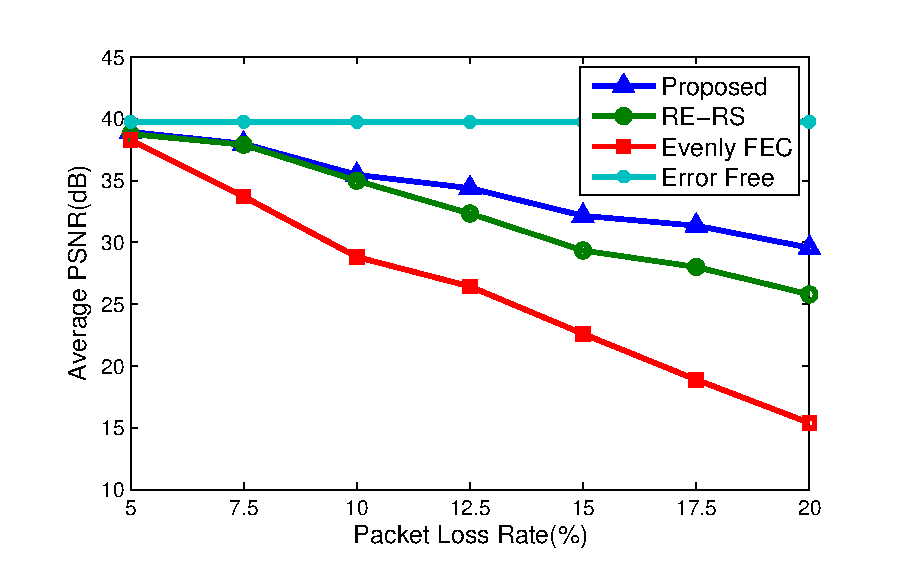
\includegraphics[width=0.7\textwidth]{loss_rate.eps}\\
  \caption{不同丢包率下PSNR表现,带宽=1Mbps,871 Kbps \emph{Foreman}序列}\label{fig:lossrate}
\end{figure}

首先,我们比较了上述三种算法在不同丢包率环境下的PSNR表现。在本实验中,我们使用了编码码率为871Kbps的\emph{Foreman}序列,网络带宽限制为1M。实验结果如图\ref{fig:lossrate}所示,其中无丢包情况的PSNR表现作为基准值标出。图中可以明显看出,我们的算法在所有丢包率情况下PSNR表现都高于其他算法,值得注意的是,随着丢包率的增大,这一差距也越来越明显。这一效果提升得益于我们的算法在不同丢包率场景下,能够通过理论计算得到最优冗余分配方案,在相同冗余率下获得更好的保护效果。当丢包率达到$20\%$时,我们的算法相比RE-RS算法获得了高达5.0 dB的PSNR增益。

\begin{figure}[htbp]
  \centering
  % Requires \usepackage{graphicx}
  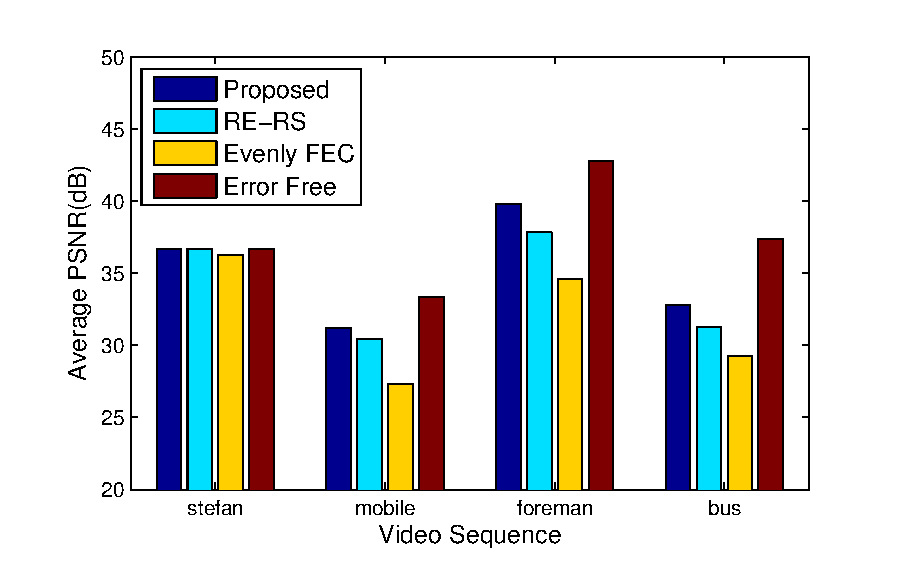
\includegraphics[width=0.7\textwidth]{videos.eps}\\
  \caption{不同视频序列下PSNR表现,带宽=2Mbps,序列:\emph{Stefan}:1441Kbps, \emph{Mobile}:1786Kbps, \emph{Foreman}:1812Kbps, \emph{Bus}:1890Kbps}\label{fig:videos}
\end{figure}

为了测试算法对不同特征视频的适应性,我们还用不同特点和码率的视频序列对三种算法的表现进行了实验。图 \ref{fig:videos} 表明,我们的算法在不同视频序列中均表现出更好的冗余保护效果。并且随着视频码率提高(同带宽下冗余率相应降低),我们的算法由于能够更有效地利用有限的冗余数据,因而获得了更明显的效果提升。

\begin{figure}[htbp]
  \centering
  % Requires \usepackage{graphicx}
  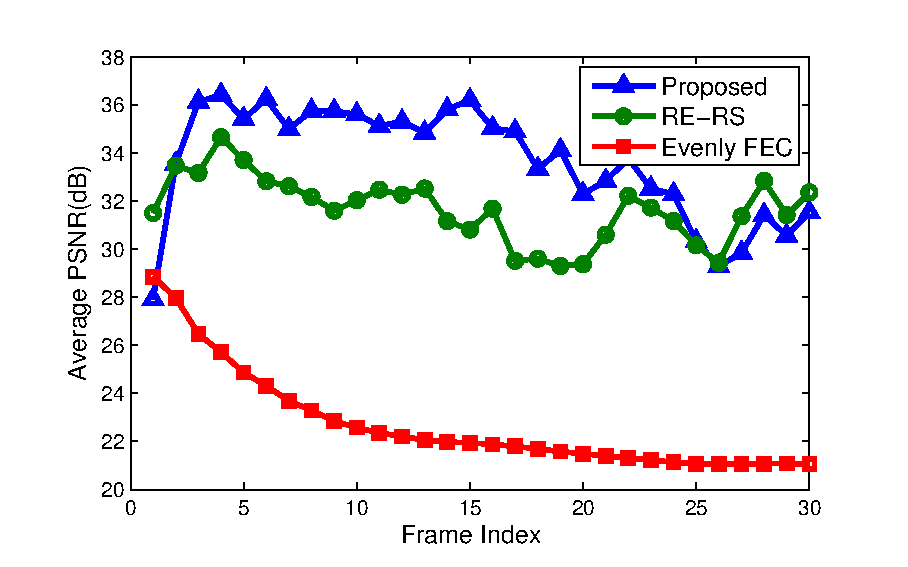
\includegraphics[width=0.7\textwidth]{uep_psnr.eps}
  \caption{逐帧PSNR表现,丢包率=$10\%$,带宽=1Mbps,871 Kbps \emph{Foreman}序列}\label{fig:psnr}
\end{figure}

最后,为了分析我们的算法在FEC冗余优化分配中的具体原理,我们对\emph{Foreman}序列在10\%丢包率,1Mbps带宽条件下进行了测试,并绘制了三种算法在GOP中每一帧的PSNR表现,如图\ref{fig:psnr}。在RE-RS和我们的算法中,由于采用了扩展窗口编码框架,视频帧间的错误传播都得到了有效控制,因此不会出现Evenly FEC这种随着帧序列增大失真明显增多的现象。而我们的算法通过在不同帧之间冗余信息的优化分配,达到了整体上失真的最小化。


\section{本章小结}
本研究中,我们对一种针对实时视频传输的扩展窗口FEC框架进行了建模、分析,并提出了一种基于此框架的冗余分配方案。我们首先针对EW-RS框架进行了准确的丢包率分析,并针对其编解码特征提出了两条推论。然后我们推导出了GOP整体语预期失真公式,作为冗余最优化分配的理论基础。在此基础上,冗余分配问题被归纳为带约束的非线性优化问题。另外,为了简化这一问题的求解,我们设计了一种基于贪心的次优求解算法,使这一冗余分配算法能够适用于实时传输场景。大量实验结果表明,我们的算法在各种网络场景下都能明显提高视频传输的FEC保护效果。
